
\section{Numerical Modeling of Heat Transfer Problem with Finite Elements Method}
\subsection{Study Domain and Mesh}
\begin{figure}
	\centering
	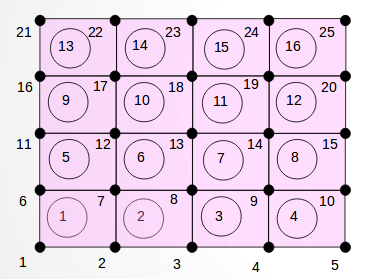
\includegraphics[height=4cm]{Images/mesh.png}
	\caption{Discretization of the domain.}
	\label{figure:mesh}
\end{figure}
\begin{mdframed}
	We want to discretize our domain in the same way described in figure \ref{figure:mesh}.
	
	The variable that we are going to use will be the \emph{length and the height of the domain}, as well as the \emph{number of the point} we want in our discretization. 
	
	A simple algorithm that takes care of that could be the one in Listing \ref{points}, where we have put in input of our function \texttt{mesh} the number of points in which we want to discretize our domain \texttt{nx,ny}.   
	\lstinputlisting[label={points},caption={Mesh}]{Matlab_Code/points.m}
	We stress the fact that in "for"~loop we take care also of the fact that if the point considered is a boundary point we have to come back and restart in \emph{another line}.
	
	The algorithm presented in Listing \ref{mesh} takes care of numbering in a proper way the elements basis and the points we have generated with the alorithm \texttt{points}.
	\lstinputlisting[label={mesh},caption={Mesh of the Domain}]{Matlab_Code/mesh.m}
\end{mdframed}
\subsection{Galerkin’s Formulation of Heat Transfer Equation}
\subsubsection{Projection of the partial differential equation on an element of the basis of the functions $ \alpha_i $}
We want to evaluate at this stage the projection of our unknown function $ T $ into the element basis $ \beta_i $, i.e., $ \forall i $ we want 
\begin{equation}
\label{eq:proj}
\iiint_{\Omega}\beta_i\nabla\cdot(-\kappa\nabla T)\diff\Omega=\iiint_{\Omega}\beta_i Q\diff\Omega
\end{equation} 
Now we can identify the element basis $ \beta_i $ with the element basis $ \alpha_i $ and so we can write  
\[\iiint_{\Omega}\alpha_i\nabla\cdot(-\kappa\nabla T)\diff\Omega=\iiint_{\Omega}\alpha_i Q\diff\Omega \]

\subsubsection{Give the weak formulation of the Galerkin’s method. Introduce the boundary conditions in the formulation.}
Using the differential identity 
\[\nabla\cdot(-\alpha_i)\kappa\nabla T)=-\alpha_i\nabla\cdot(\kappa\nabla T)-\kappa\nabla\alpha_i\nabla T\]
we can plug the above equation into \eqref{eq:proj} obtaining 

\[\iiint_{\Omega}\nabla\cdot(-\alpha_i)\kappa\nabla T\diff\Omega+\iiint_{\Omega}\kappa\nabla\alpha_i\nabla T\diff\Omega=\iiint_{\Omega}\alpha_i Q\diff\Omega\]

By the way, we have, thanks to the divergnece theorem, that 
\[\iiint_{\Omega}\nabla\cdot(-\alpha_i)\kappa\nabla T\diff\Omega=-\iint_{\Gamma}\alpha_i\kappa\nabla T\cdot\vec{n}\diff\Gamma. \]

Then finally we have the \textbf{weak formulation of the problem} \eqref{eq:proj}
\[ \iiint_{\Omega}\kappa\nabla\alpha_i\nabla T\diff\Omega-\iint_{\Gamma}\alpha_i\kappa\nabla T\cdot\vec{n}\diff\Gamma=\iiint_{\Omega}\alpha_i Q\diff\Omega. \]
\medskip

Introducing the boundary conditions, see \eqref{problem:heat}, we have
\[\begin{cases}
-\kappa\nabla T\cdot \vec{n}=h(T-T_r),& \text{on the free surface}\\
-\kappa\nabla T\cdot \vec{n}=0,&\text{on all the non-free surface}\\
\end{cases}\]
and then 
\begin{equation}
\forall i \iint_{\Gamma}\alpha_i h(T-T_r)\diff\Gamma+\iiint_{\Omega}\kappa\nabla\alpha_i\nabla T\diff\Omega =\iiint_{\Omega}\alpha_i Q\diff\Omega
\end{equation}


\subsubsection{Precise the expression of the elementary volume, the elementary surface for respectively the volume integral and surface integral.}
The idea is to transform an integral all over the volume $ \Omega $ in many sums all over the small elements $ e $. The elements must be disjoint pairwise and the union of the small elements $ e $ must be give the original volume $ \Omega $. In symbols we have
\[\iiint_{\Omega}\left[\dots\right]\diff\Omega=\sum_e\iiint_{\omega_e}\left[\dots\right]\diff\Omega_e \]
Similarly we'll have that the integral all over the susface is made up by the sum by the sum of all the small surfaces:
\[\iint_{\Gamma}\left[\dots\right]\diff\Gamma=\sum_f\iint_{\gamma_f}\left[\dots\right]\diff\Gamma_f \] 

We use the canonical change of variable, from cartesian to cylindrical, i.e., \begin{align}\label{change}
(x,y,z)&\to(r,\theta,z)\\
(x,y,z)&\mapsto(rcos(\theta),rsin(\theta),z)\nonumber
\end{align}
The change of variable given by Eq.\ref{change} gives as determinant of the Jacobian matrix the element $ r $, in such a way that the integration must be performed changing $ \diff x\diff y\diff z $ into $ r\diff r\diff\theta\diff z $.

Then we have that 
\[ 2\pi\iint_{\Omega}\kappa\nabla\alpha_i\nabla T\,r\diff r\diff z-2\pi\int_{\Gamma}\alpha_i\kappa\nabla T\cdot\vec{n}\diff z=2\pi\iint_{\Omega}\alpha_i Q\,r\diff r\diff z. \]

\subsubsection{Give the expression of the integrals on the reference element}
The expression for each element of the basis is then
\[\sum_j \iiint_{e}\nabla\alpha_i\nabla\alpha_j\xi\diff\xi\diff\eta. \] 

Let's notice that we have 
\[T=\sum_{j=1}^N\alpha_j(\xi,\eta,\zeta)\cdot T_j \]
and so the differential becomes
\[\nabla T=\sum_{j=1}^N\nabla\alpha_j(\xi,\eta,\zeta)\cdot T_j \]
where through elementary calculations we can see that 
\[\nabla \alpha_j=\begin{bmatrix} Jac J \end{bmatrix}^{-1}\begin{bmatrix}
\pd{\alpha}{\xi}\\\pd{\alpha}{\eta}\\\pd{\alpha}{\zeta} 
\end{bmatrix}. \]

Then the final expression will be
\begin{align*}
\sum_e\iint_{\omega_e}\kappa\nabla\alpha_i\cdot\left(\sum_{j=1}^{N}\nabla\alpha_jT_j \right) \xi\diff\xi\diff\eta +\sum_f\int_{\Gamma}\alpha_ih\left(\sum_{j=1}^{N}\alpha_jT_j\right)\diff \eta=
\sum_f\int_{\Gamma}\alpha_ihT_r\diff \eta+\sum_e\iiint_{\omega_e}\alpha_iQ\,\xi\diff\xi\diff\eta.
\end{align*}
 

\subsubsection{Detail the expression of the elementary matrix on an element $ e $. Precise the size of each elementary matrix (sub matrix). Precise the expression of each integral and the principle of calculation. For each integral, precise the nature of the element $ e $} 

The elementary matrix of an element $ e $ is given by the inner product $ \nabla\alpha_i\nabla\alpha_j $. In particular we'll have a matrix $ A_{ij}^e $ in which we will have in position $ (i,j) $ the element $ \nabla\alpha_i\nabla\alpha_j $. 


The matrix $ A_{ij}^e $ is a $ 4\times4 $ matrix, for each inner element. For the outer element it will be a $ 3\times3 $ or $ 2\times2 $ depending on the position. 
\begin{figure}
	\centering
	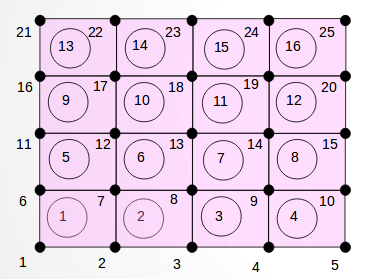
\includegraphics[height=4cm]{Images/mesh.png}
	\caption{The boundary elements will have 3 boundaries or 2, depending on which one we are considering.}
\end{figure}

\subsubsection{Detail the elementary second term on an element $ e $. Precise the size of each elementary second vector. Precise the expression of each integral and the principle of calculation. Precise the principle of the construction of the matrix system. For each integral, precise the nature of the element $ e $} 

\subsubsection{Precise the principle of the construction of the matrix and the second term vector of the system}
